\documentclass[paper=a4, fontsize=11pt]{scrartcl}
\usepackage[T1]{fontenc}  % proper encoding for output file
\usepackage[utf8]{inputenc}  % except UTF-8 character in source
\usepackage[english]{babel}  % set document language
\usepackage{amsmath,amsfonts,amsthm}  % math type setting
\usepackage{mhchem}  % chemical expressions
\usepackage{graphicx}  % inclue graphics
\usepackage{url}
\usepackage{caption}
\usepackage{subcaption}
\setlength\parindent{0pt} % Removes all indentation from paragraphs

% Macro to conveniently typeset chemical symbols.
\newcommand{\symb}[1]{$\,\mathrm{#1}$}


\title{Exercise 8: Optimal Estimation Method}
\author{Sample Solution}
\date{Effective: 16.01.2019}

%%%%%%%%%%%%%%%%%%%%%%%%%%%%%%%%%%%%%%%%%%%%%%%%%%%%%%%%%%%%%%%%%%%%%%%%%%%%%%%
\begin{document}

\maketitle

2. Plot both the measured spectrum and the simulated a priori spectrum as a
function of the frequency grid. Add reasonable labels to your plots.

\begin{figure}[ht]
  \centering
  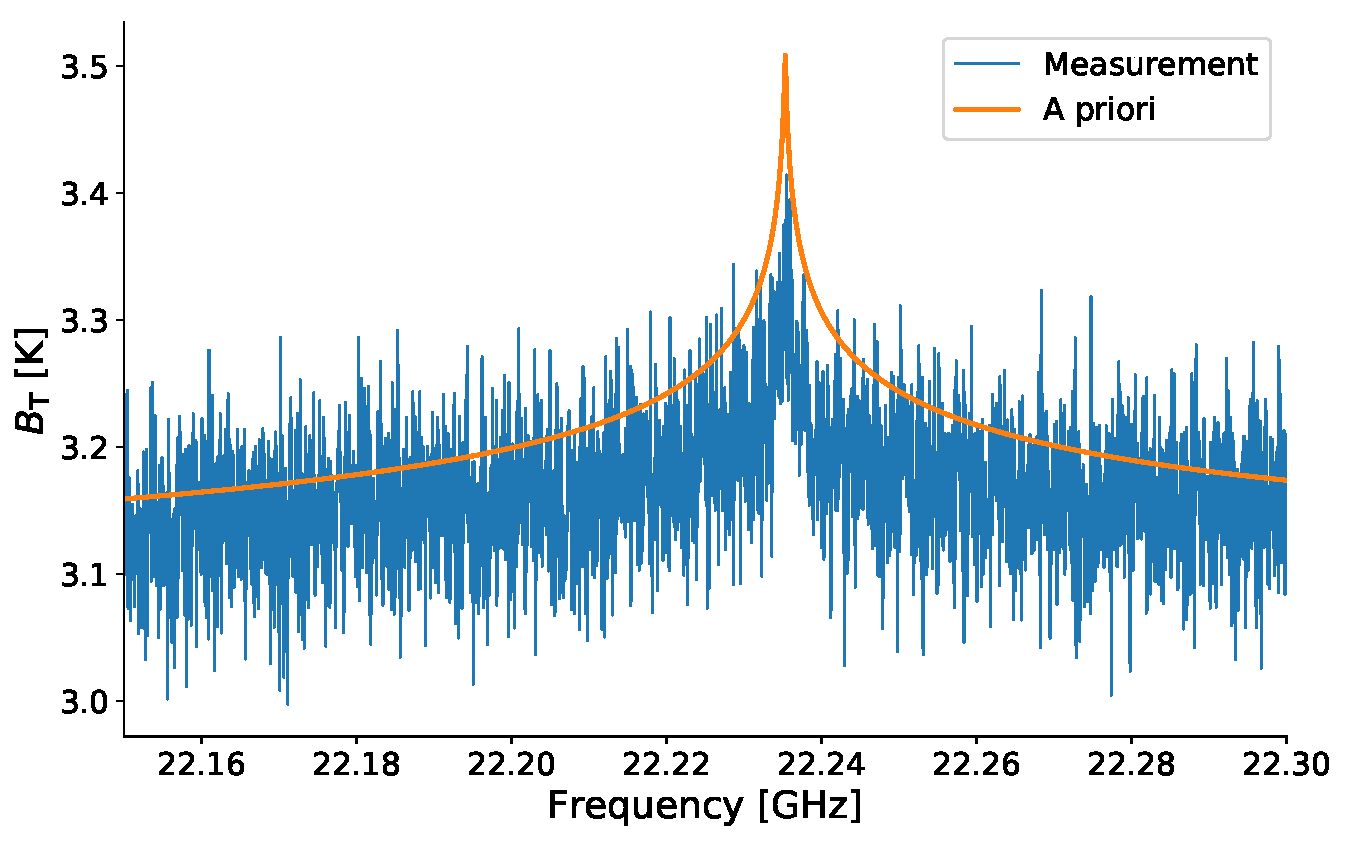
\includegraphics[width=\textwidth]{plots/bt_spectrum.pdf}
  \caption{Brightness temperature \label{fig:bt_spectrum}}
\end{figure}

\newpage

3. Plot the Jacobians K in a suitable way.

\begin{figure}[ht]
  \centering
  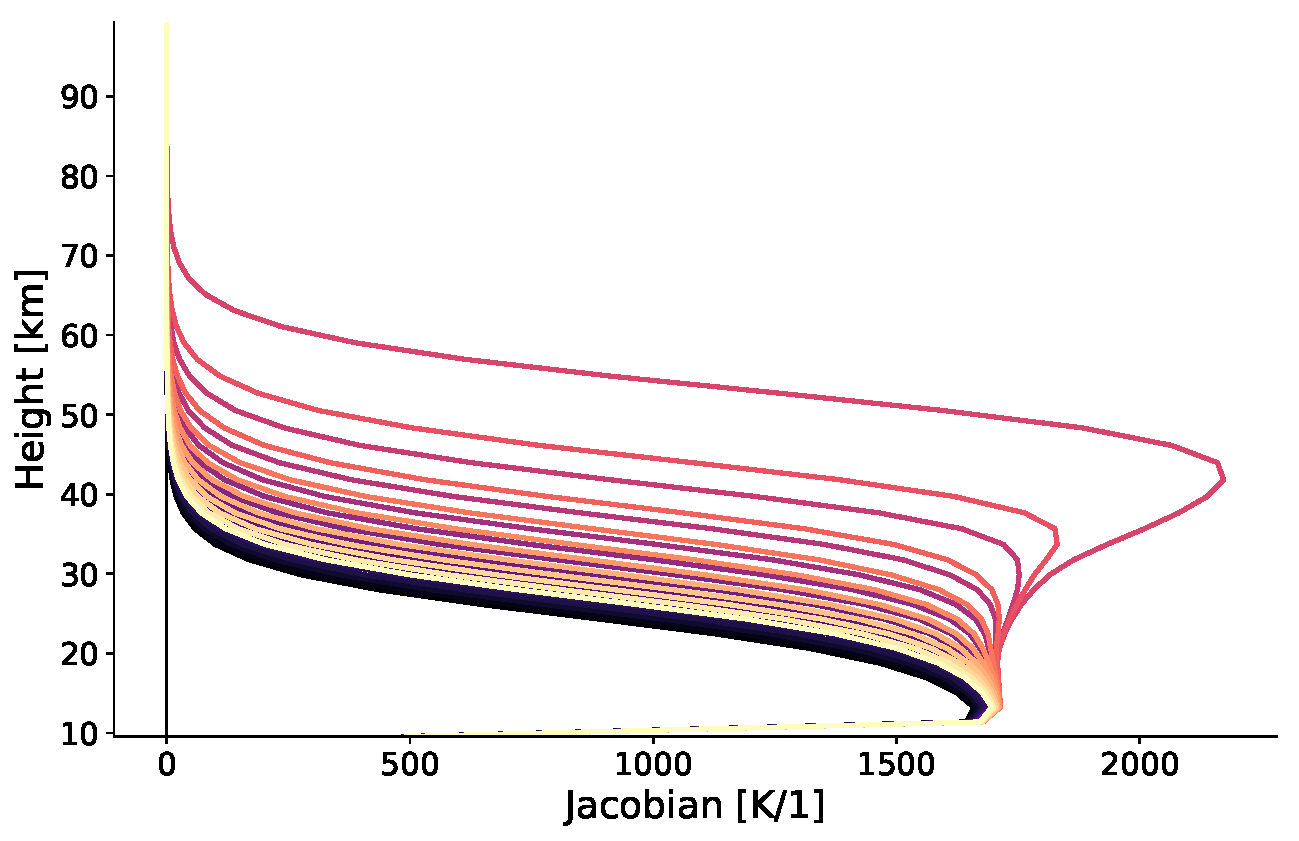
\includegraphics[width=\textwidth]{plots/jacobians.pdf}
  \caption{Jacobians \label{fig:jacobians}}
\end{figure}

\newpage

5. Plot the retrieved water vapor profile alongside the a priori state and the
true atmospheric state as a function of height. Discuss the results.
\begin{itemize}
  \item The OEM retrieval is able to reproduce the general water vapor profile
    up to around 60\,km.
  \item There is no information above 70\,km, the solution is equal to the a
    priori.
  \item The oscillating shape of the true water vapor profile is noticable
    between 20--40\,km in the retrieval.
\end{itemize}

\begin{figure}[ht]
  \centering
  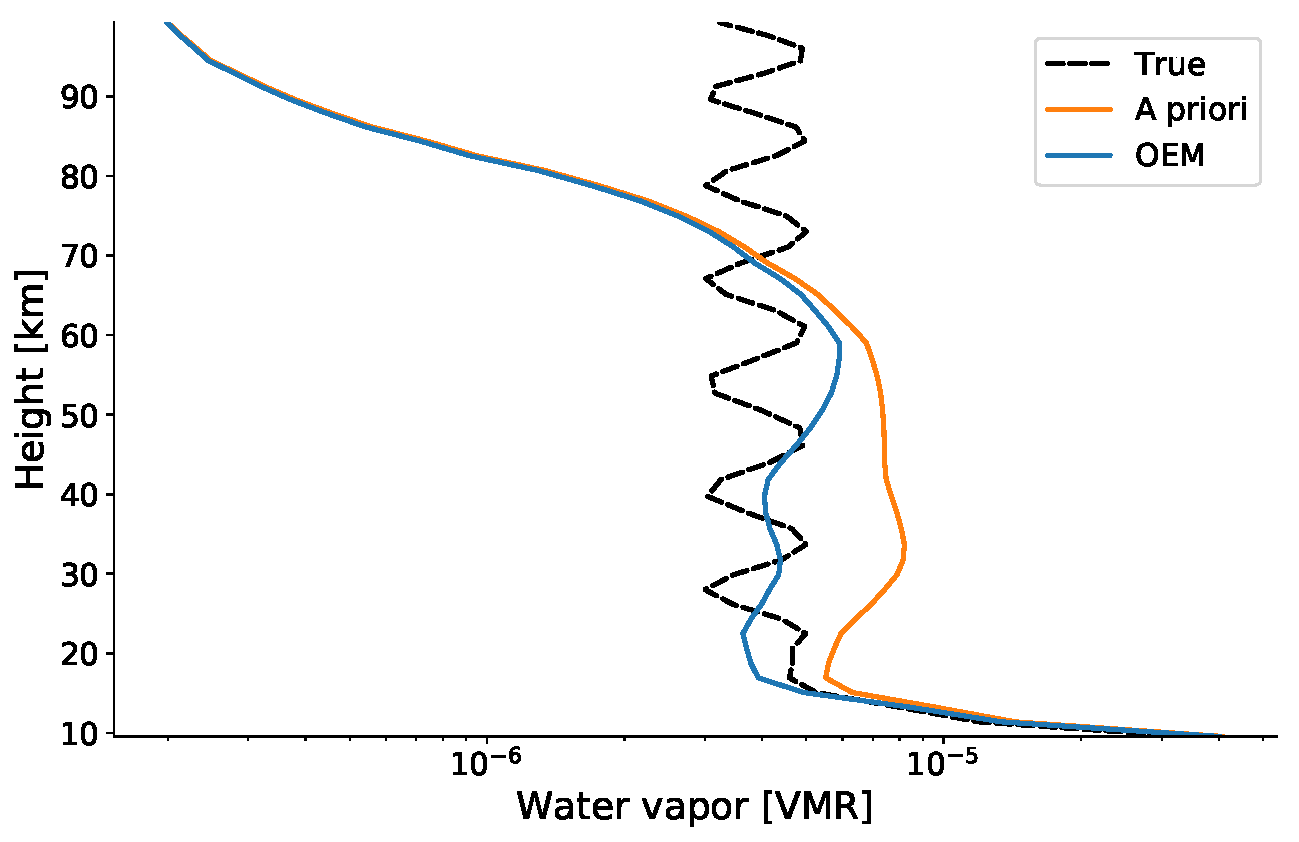
\includegraphics[width=\textwidth]{plots/water_vapor_profile.pdf}
  \caption{Water vapor profile \label{fig:wv_profile}}
\end{figure}

\newpage

6. Plot the columns (kernels) as a function of height and interpret the result.
7. Calculate the measurement response and plot it together with the averaging
kernels. In wich heights does the measurement provide useful information? Is it
possible to estimate the vertical resolution?
\begin{itemize}
  \item The measurement response indicates useful information between
    15--60\,km
  \item The width (overlap) of the averaging kernels allow to estimate the
    vertical resolution. The vertical resolution decreases with height, which
    is consistent with the retrieved water vapor profile (the oscillation shape
    is no longer retrieved).
\end{itemize}

\begin{figure}[ht]
  \centering
  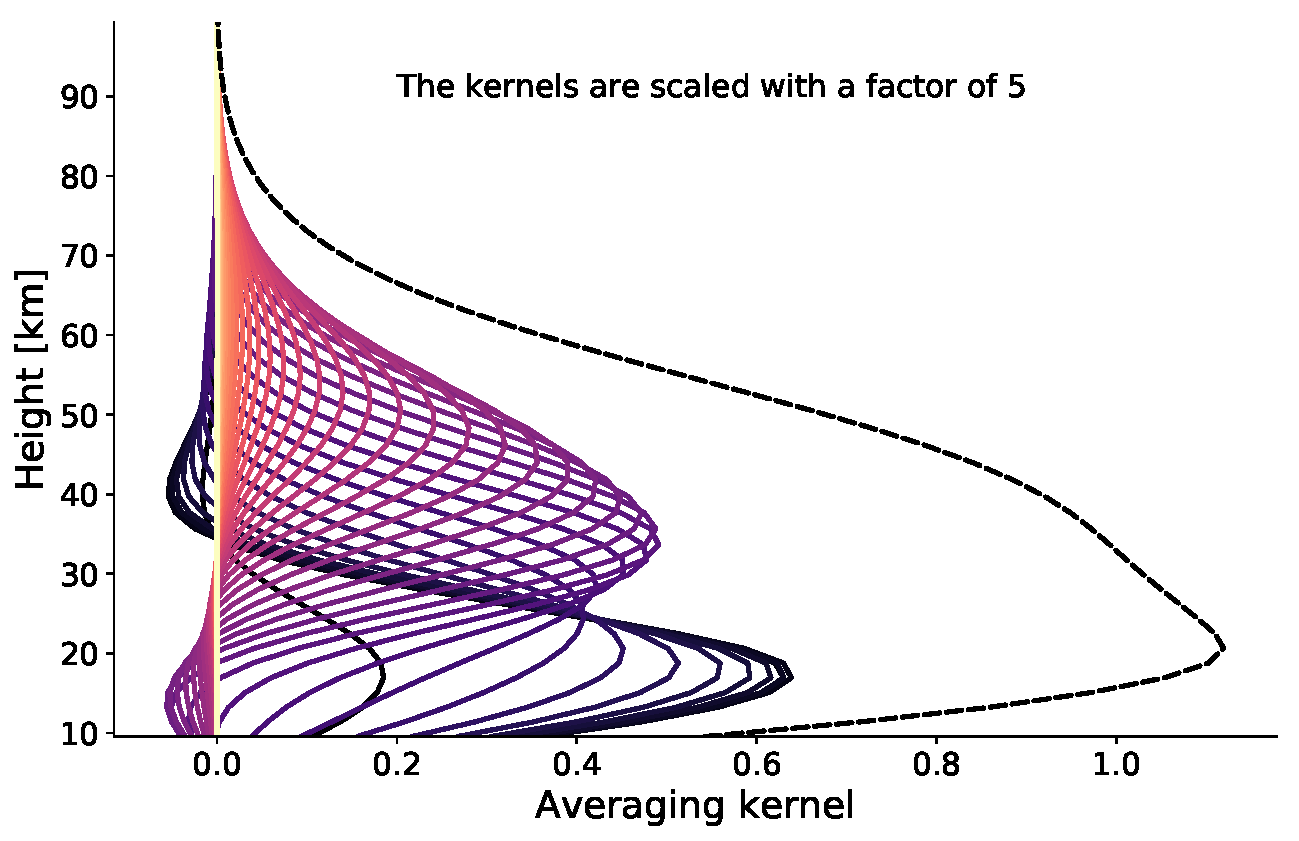
\includegraphics[width=\textwidth]{plots/averaging_kernels.pdf}
  \caption{Averaging kernels \label{fig:averaging_kernels}}
\end{figure}

\end{document}
